\chapter{Specifikacija programske potpore}
		
	\section{Funkcionalni zahtjevi}
			
			\textbf{\textit{dio 1. revizije}}\\
			
			\textit{Navesti \textbf{dionike} koji imaju \textbf{interes u ovom sustavu} ili  \textbf{su nositelji odgovornosti}. To su prije svega korisnici, ali i administratori sustava, naručitelji, razvojni tim.}\\
				
			\textit{Navesti \textbf{aktore} koji izravno \textbf{koriste} ili \textbf{komuniciraju sa sustavom}. Oni mogu imati inicijatorsku ulogu, tj. započinju određene procese u sustavu ili samo sudioničku ulogu, tj. obavljaju određeni posao. Za svakog aktora navesti funkcionalne zahtjeve koji se na njega odnose.}\\
			
			
			\noindent \textbf{Dionici:}
			
			\begin{packed_enum}
				
				\item Administrator
				\item Neregistrirani korisnik/posjetitelj			
				\item Registrirani korisnik/posjetitelj
				
			\end{packed_enum}
			
			\noindent \textbf{Aktori i njihovi funkcionalni zahtjevi:}
			
			
			\begin{packed_enum}
				\item  \underbar{Administrator (inicijator) može:}
				
				\begin{packed_enum}
					
					\item dodati autore i radove
					\item kreirati stručne konferencije
					\item izabirati fotografije koje su slikane tijekom konferencije
					\item objaviti rezultate konferencije
					
				\end{packed_enum}
			
				\item  \underbar{Neregistrirani korisnik (inicijator) može:}
				
				\begin{packed_enum}
					
					\item unijeti lozinku za pristup sustavu
					\item registrirati se u sustav
					
				\end{packed_enum}
				
				
				\item  \underbar{Registrirani korisnik (inicijator) može:}
				
				\begin{packed_enum}
					
					\item pregledavati promotivne materijale pokrovitelja konferencije
					\item pregledavati radove/postere sudionika
					\item ocjenjivati radove svakog pojedinca
					\item uz pomoć direktnog video praćenja pratiti trenutna događanja u glavnoj konferencijskoj dvorani
					\item glasati za svaki pojedini rad/poster
					\item vidjeti konačne reultate konferencije
					\item dobiti pozivnicu na mail za dodjelu nagrade za prva tri nagrađena rada
					\item pregledavati i spremati fotografije koje su fotografirane tijekom konferencije
					\item vidjeti mjesto održavanje konferencije i podatke o trenutnim vremenskim uvjetima
					
				\end{packed_enum}
					
				\item  \underbar{Baza podataka (sudionik) obavlja:}
					
					\begin{packed_enum}
						
						\item pohranjuje sve podatke o korisnicima
						\item pohranjuje sve podatke o autorima i njihovim radovima
						\item pohranjuje sve podatke o glasovima
						\item pohranjuje sve podatke o fotografija slikanim tijekom konferencije
						
					\end{packed_enum}
				
			\end{packed_enum}
			
			\eject 
			
			
				
			\subsection{Obrasci uporabe}
				
				\textbf{\textit{dio 1. revizije}}
				
				\subsubsection{Opis obrazaca uporabe}
				
					\noindent \underbar{\textbf{UC$<$broj obrasca$>$ -$<$ime obrasca$>$}}
					\begin{packed_item}
	
						\item \textbf{Glavni sudionik: }$<$sudionik$>$
						\item  \textbf{Cilj:} $<$cilj$>$
						\item  \textbf{Sudionici:} $<$sudionici$>$
						\item  \textbf{Preduvjet:} $<$preduvjet$>$
						\item  \textbf{Opis osnovnog tijeka:}
						
						\item[] \begin{packed_enum}
	
							\item $<$opis korak jedan$>$
							\item $<$opis korak dva$>$
							\item $<$opis korak tri$>$
							\item $<$opis korak četiri$>$
							\item $<$opis korak pet$>$
						\end{packed_enum}
						
						\item  \textbf{Opis mogućih odstupanja:}
						
						\item[] \begin{packed_item}
	
							\item[2.a] $<$opis mogućeg scenarija odstupanja u koraku 2$>$
							\item[] \begin{packed_enum}
								
								\item $<$opis rješenja mogućeg scenarija korak 1$>$
								\item $<$opis rješenja mogućeg scenarija korak 2$>$
								
							\end{packed_enum}
							\item[2.b] $<$opis mogućeg scenarija odstupanja u koraku 2$>$
							\item[3.a] $<$opis mogućeg scenarija odstupanja  u koraku 3$>$
							
						\end{packed_item}
					\end{packed_item}
					
					\noindent \underbar{\textbf{UC1 - Registracija}}
					\begin{packed_item}
						
						\item \textbf{Glavni sudionik: }Korisnik
						\item  \textbf{Cilj:} Registrirati se u sustavu kako bi se omogućio pristup svim funkcionalnostima aplikacije.
						\item  \textbf{Sudionici:} Baza podataka
						\item  \textbf{Preduvjet:} Posjetitelj ima dobivenu lozinku, pristup internetu i otvoren je za registraciju.
						\item  \textbf{Opis osnovnog tijeka:}
						
						\item[] \begin{packed_enum}
							
							\item Posjetitelj pristupa registracijskoj stranici aplikacije.
							\item Posjetitelj unosi svoje osobne podatke za registraciju.
							\item Sustav provjerava podatke i stvara račun za posjetitelja.
							\item Posjetitelj prima potvrdu o uspješnoj registraciji.
						\end{packed_enum}
						
						\item  \textbf{Opis mogućih odstupanja:}
						
						\item[] \begin{packed_item}
							
							\item[3.a] Ako su uneseni podaci nepotpuni ili neispravni:
							\item[] \begin{packed_enum}
								
								\item Sustav prikazuje upozorenje i traži ispravak podataka.
								
							\end{packed_enum}
						\end{packed_item}
					\end{packed_item}
					
					\noindent \underbar{\textbf{UC2 - Prijava u sustav}}
					\begin{packed_item}
						
						\item \textbf{Glavni sudionik: }Korisnik
						\item  \textbf{Cilj:} Prijaviti se u sustav kako bi se pristupilo svim funkcionalnostima aplikacije.
						\item  \textbf{Sudionici:} Baza podataka
						\item  \textbf{Preduvjet:} Posjetitelj je već registriran u sustavu.
						\item  \textbf{Opis osnovnog tijeka:}
						
						\item[] \begin{packed_enum}
							
							\item Posjetitelj pristupa stranici za prijavu u aplikaciju.
							\item Posjetitelj unosi svoje korisničko ime i lozinku.
							\item Sustav provjerava unesene podatke i omogućuje pristup.
						\end{packed_enum}
						
						\item  \textbf{Opis mogućih odstupanja:}
						
						\item[] \begin{packed_item}
							
							\item[3.a] Ako su uneseni podaci netočni:
							\item[] \begin{packed_enum}
								
								\item Sustav prikazuje upozorenje o neuspjeloj prijavi.
								
							\end{packed_enum}

						\end{packed_item}
					\end{packed_item}
					
					\noindent \underbar{\textbf{UC3 -  Glasovanje za svaki pojedini poster}}
					\begin{packed_item}
						
						\item \textbf{Glavni sudionik: }Korisnik
						\item  \textbf{Cilj:} Glasovati za određeni poster na konferenciji.
						\item  \textbf{Sudionici:} Baza podataka, poster
						\item  \textbf{Preduvjet:} Posjetitelj je prijavljen u sustavu i vrijeme je glasanja.
						\item  \textbf{Opis osnovnog tijeka:}
						
						\item[] \begin{packed_enum}
							
							\item Posjetitelj pregledava dostupne postere.
							\item Posjetitelj odabire poster za glasovanje.
							\item Sustav bilježi glas posjetitelja za odabrani poster.
							
						\end{packed_enum}
						
						\item  \textbf{Opis mogućih odstupanja:}
						
						\item[] \begin{packed_item}
							
							\item[2.a] Posjetitelj je već glasovao.
							\item[] \begin{packed_enum}
								
								\item Sustav pokazuje upozorenje da je moguće samo jednom glasovati.
								
							\end{packed_enum}
							
						\end{packed_item}
					\end{packed_item}
					
					\noindent \underbar{\textbf{UC4 - Pregled radova sudionika}}
					\begin{packed_item}
						
						\item \textbf{Glavni sudionik: }Korisnik
						\item  \textbf{Cilj:} Pregledati radove sudionika konferencije.
						\item  \textbf{Sudionici:} Baza podataka
						\item  \textbf{Preduvjet:} Posjetitelj je prijavljen u sustavu.
						\item  \textbf{Opis osnovnog tijeka:}
						
						\item[] \begin{packed_enum}
							
							\item Posjetitelj pristupa dijelu aplikacije koji prikazuje sve dostupne radove sudionika.
							\item Posjetitelj pregledava pojedinačne radove i postere.

						\end{packed_enum}
						
						\item  \textbf{Opis mogućih odstupanja:}
						
						\item[] \begin{packed_item}
							
							\item Nema mogućih odstupanja za ovaj obrazac uporabe.
							
						\end{packed_item}
					\end{packed_item}
					
					\noindent \underbar{\textbf{UC5 - Prijava autora, radova i postera}}
					\begin{packed_item}
						
						\item \textbf{Glavni sudionik: }Administrator
						\item  \textbf{Cilj:} Dodati autora i njegov rad u bazu podataka.
						\item  \textbf{Sudionici:} Baza podataka, autor
						\item  \textbf{Preduvjet:} Administrator ima sve ovlasti za upravljanje bazom podataka te je autor podnio ispravnu prijavnicu.
						\item  \textbf{Opis osnovnog tijeka:}
						
						\item[] \begin{packed_enum}
							
							\item Autor elektroničkom poštom šalje administratoru sve potrebne informacije, to uključuje ime autora, rad i poster.
							\item Administrator dodaje autora i njegov rad te poster u bazu podataka.
					
						\end{packed_enum}
						
						\item  \textbf{Opis mogućih odstupanja:}
						
						\item[] \begin{packed_item}
							
							\item[1.a] Autor nije poslao svoje ime ili svoj rad.
							\item[] \begin{packed_enum}
								
								\item Administrator obještava autora da nije poslao sve potrebne informacije.
								
							\end{packed_enum}
							
						\end{packed_item}
					\end{packed_item}
					
					\noindent \underbar{\textbf{UC6 - Dobivanje lozinke za pristup sustavu}}
					\begin{packed_item}
						
						\item \textbf{Glavni sudionik: }Neregistrirani korisnik
						\item  \textbf{Cilj:} Dobiti pristup sustavu.
						\item  \textbf{Sudionici:} Baza podataka
						\item  \textbf{Preduvjet:} Biti sudionik konferencije.
						\item  \textbf{Opis osnovnog tijeka:}
						
						\item[] \begin{packed_enum}
							
							\item Dolazak na stručnu konferenciju.
							\item Dolazak na recepciju i dobivanje lozinke za pristup sustavu.
							\item Unos lozinke u sustav.

						\end{packed_enum}
						
						\item  \textbf{Opis mogućih odstupanja:}
						
						\item[] \begin{packed_item}
							
							\item[3.a] Neispravna lozinka.
							\item[] \begin{packed_enum}
								
								\item Sustav obavještava korisnika o neispravnoj lozinci
								
							\end{packed_enum}
							
						\end{packed_item}
					\end{packed_item}
					
					\noindent \underbar{\textbf{UC7 - Objava rezultata}}
					\begin{packed_item}
						
						\item \textbf{Glavni sudionik: }Administrator
						\item  \textbf{Cilj:} Objaviti rezultate konferencije.
						\item  \textbf{Sudionici:} Baza podataka, registrirani korisnici.
						\item  \textbf{Preduvjet:} Završeno glasanje, administrator je prijavljen.
						\item  \textbf{Opis osnovnog tijeka:}
						
						\item[] \begin{packed_enum}
							
							\item Završetak glasanja.
							\item Administrator provjerava ispravnost glasova u bazi podataka.
							\item Unos rezultata u web aplikaciju.
							\item Registrirani korisnici sada na glavnoj stranici mogu vidjeti rezultate.
						\end{packed_enum}
						
						\item  \textbf{Opis mogućih odstupanja:}
						
						\item[] \begin{packed_item}
							
							\item Nema mogućih odstupanja za ovaj obrazac uporabe.
							
						\end{packed_item}
					\end{packed_item}
					
					\noindent \underbar{\textbf{UC8 - Slanje obavijest autorima o njihovom uspjehu i pozivnice na dodjelu nagrade}}
					\begin{packed_item}
						
						\item \textbf{Glavni sudionik: }Administrator
						\item  \textbf{Cilj:} Poslati e-mail autorima o njihovom uspjehu i pozivnicu na dodjelu nagrade za prva tri rada.
						\item  \textbf{Sudionici:} Baza podataka, autori, registrirani korisnici
						\item  \textbf{Preduvjet:} Administrator ima pristup bazi podataka, završeno glasanje, objavljeni su rezultati glasanja.
						\item  \textbf{Opis osnovnog tijeka:}
						
						\item[] \begin{packed_enum}
							
							\item Administrator šalje mail svim autorima, koji sadrži njihov rang prema glasovima posjetitelja i pozivnicu na dodjelu nagrada.
						\end{packed_enum}
						
						\item  \textbf{Opis mogućih odstupanja:}
						
						\item[] \begin{packed_item}
							
							\item Nema mogućih odstupanja za ovaj obrazac uporabe.
							
						\end{packed_item}
					\end{packed_item}
					
					\noindent \underbar{\textbf{UC9 - Slanje pozivnice za dodjelu nagrade za prva tri nagrađena rada}}
					\begin{packed_item}
						\item \textbf{Glavni sudionik:} Sistemski administrator
						\item \textbf{Cilj:} Slanje pozivnice autorima nagrađenih radova za dodjelu nagrade.
						\item \textbf{Sudionici:} Autori nagrađenih radova
						\item \textbf{Preduvjet:} Administrator je pregledao rezultate glasovanja i odabrao nagrađene radove.
						\item \textbf{Opis osnovnog tijeka:}
						
						\begin{packed_enum}
							\item Sistemski administrator pristupa opciji "Slanje pozivnice za dodjelu nagrade" u aplikaciji.
							\item Administrator odabire autore nagrađenih radova.
							\item Sistem šalje pozivnice autorima nagrađenih radova za dodjelu nagrade.
						\end{packed_enum}
						
						\item \textbf{Opis mogućih odstupanja:}
						
						\begin{packed_item}
							\item[2.a] Administrator odustaje od slanja pozivnica.
						\end{packed_item}
					\end{packed_item}
					
					
					\noindent \underbar{\textbf{UC10 - Pregled fotografija (koje su slikane tijekom konferencije)}}
					\begin{packed_item}
						\item \textbf{Glavni sudionik:} Registrirani korisnici
						\item \textbf{Cilj:} Pregledati fotografije snimljene tijekom konferencije.
						\item \textbf{Sudionici:} Baza podataka
						\item \textbf{Preduvjet:} Korisnik je prijavljen u sustav i ima pristup fotografijama.
						\item \textbf{Opis osnovnog tijeka:}
						
						\begin{packed_enum}
							\item Korisnik pristupa dijelu aplikacije koji prikazuje dostupne fotografije s konferencije.
							\item Korisnik pregledava dostupne fotografije.
						\end{packed_enum}
						
						\item \textbf{Opis mogućih odstupanja:}
						
						\begin{packed_item}
							\item Nema mogućih odstupanja za ovaj slučaj uporabe.
						\end{packed_item}
					\end{packed_item}
					
					
					\noindent \underbar{\textbf{UC11 - Spremanje fotografija na svoj uređaj}}
					\begin{packed_item}
						\item \textbf{Glavni sudionik:} Registrirani korisnici
						\item \textbf{Cilj:} Spremiti odabrane fotografije na svoj uređaj.
						\item \textbf{Sudionici:} Baza podataka
						\item \textbf{Preduvjet:} Korisnik je prijavljen u sustav i pregledava fotografije.
						\item \textbf{Opis osnovnog tijeka:}
						
						\begin{packed_enum}
							\item Korisnik pregledava fotografije i odabire opciju "Označi" za fotografije koje želi spremiti.
							\item Korisnik potvrđuje opciju "Spremi na uređaj".
							\item Sustav preuzima odabrane fotografije i sprema ih na uređaj korisnika.
						\end{packed_enum}
						
						\item \textbf{Opis mogućih odstupanja:}
						
						\begin{packed_item}
							\item Korisnik može odustati od spremanja fotografija odabirom opcije "Odustani".
						\end{packed_item}
					\end{packed_item}
					
					
					\noindent \underbar{\textbf{UC12 - Direktno video praćenje konferencije}}
					\begin{packed_item}
						\item \textbf{Glavni sudionik:} Registrirani korisnici
						\item \textbf{Cilj:} Mogućnost praćenja video prijenosa događanja konferencije u stvarnom vremenu.
						\item \textbf{Sudionici:} Baza podataka, konferencija
						\item \textbf{Preduvjet:} Korisnik je prijavljen u sustav i ima stabilnu internetsku vezu.
						\item \textbf{Opis osnovnog tijeka:}
						
						\begin{packed_enum}
							\item Registrirani korisnik pristupa opciji "Direktno video praćenje" u aplikaciji.
							\item Sustav prikazuje dostupne video prijenose događanja konferencije.
							\item Korisnik odabire željeni video prijenos za praćenje.
						\end{packed_enum}
						
						\item \textbf{Opis mogućih odstupanja:}
						
						\begin{packed_item}
							\item[2.a] Ako korisnik nema stabilnu internetsku vezu:
							\begin{packed_enum}
								\item Sustav obavještava korisnika da je potrebna stabilna internetska veza za praćenje video prijenosa.
							\end{packed_enum}
						\end{packed_item}
					\end{packed_item}
					
					\noindent \underbar{\textbf{UC13 - Slanje potrebnih materijala sistemskom administratoru za prijavu na konferenciju}}
					\begin{packed_item}
						\item \textbf{Glavni sudionik:} Autori konferencijskih radova
						\item \textbf{Cilj:} Poslati potrebne materijale sistemskom administratoru kako bi se prijavili na konferenciju.
						\item \textbf{Sudionici:} Sistemski administrator, baza podataka
						\item \textbf{Preduvjet:} Autori su registrirani u sustavu.
						\item \textbf{Opis osnovnog tijeka:}
						
						\begin{packed_enum}
							\item Autori pristupaju opciji za slanje materijala u aplikaciji.
							\item Autori šalju potrebne materijale, poput radova i postera, elektroničkom poštom u aplikaciji.
							\item Sistemski administrator prima materijale i provjerava prijave radova autora.
						\end{packed_enum}
						
						\item \textbf{Opis mogućih odstupanja:}
						
						\begin{packed_item}
							\item[2.a] Ako su poslani materijali nepotpuni ili neispravni:
							\begin{packed_enum}
								\item Sistemski administrator obavještava autore o problemima s poslanim materijalima i traži ispravke.
							\end{packed_enum}
						\end{packed_item}
					\end{packed_item}
					
				
					
				\subsubsection{Dijagrami obrazaca uporabe}
					
					\textit{Prikazati odnos aktora i obrazaca uporabe odgovarajućim UML dijagramom. Nije nužno nacrtati sve na jednom dijagramu. Modelirati po razinama apstrakcije i skupovima srodnih funkcionalnosti.}
					
					\begin{figure}[H]
						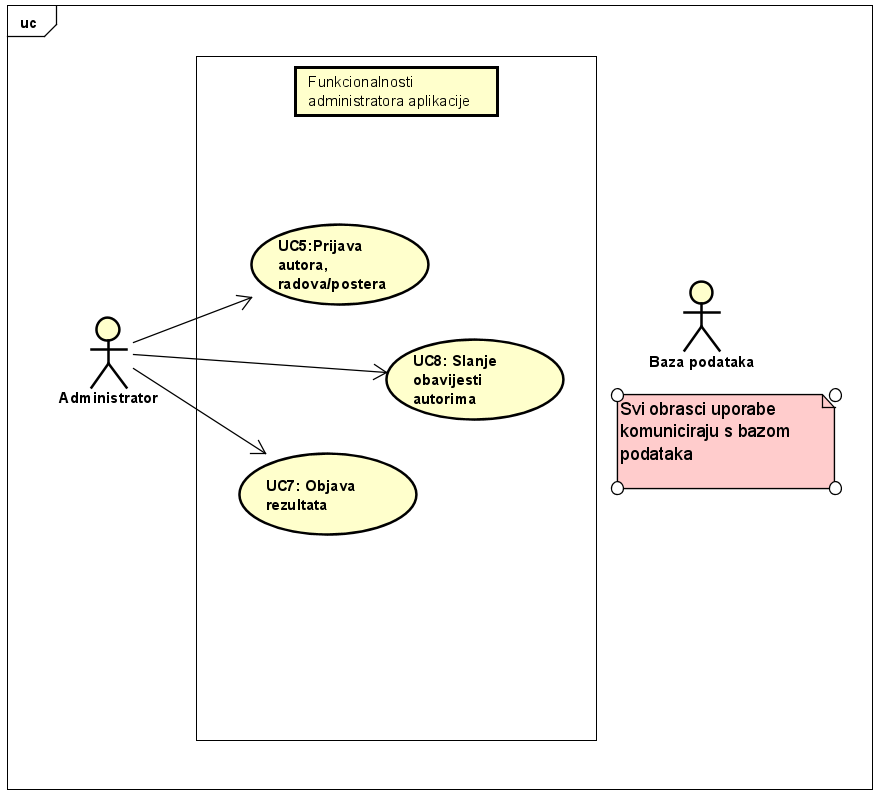
\includegraphics[scale=0.6]{slike/uc dijagram admin.PNG} %veličina slike u odnosu na originalnu datoteku i pozicija slike
						\centering
						\caption{Dijagram obrazaca uporabe - administrator}
						\label{fig:promjene}
					\end{figure}
					\begin{figure}[H]
						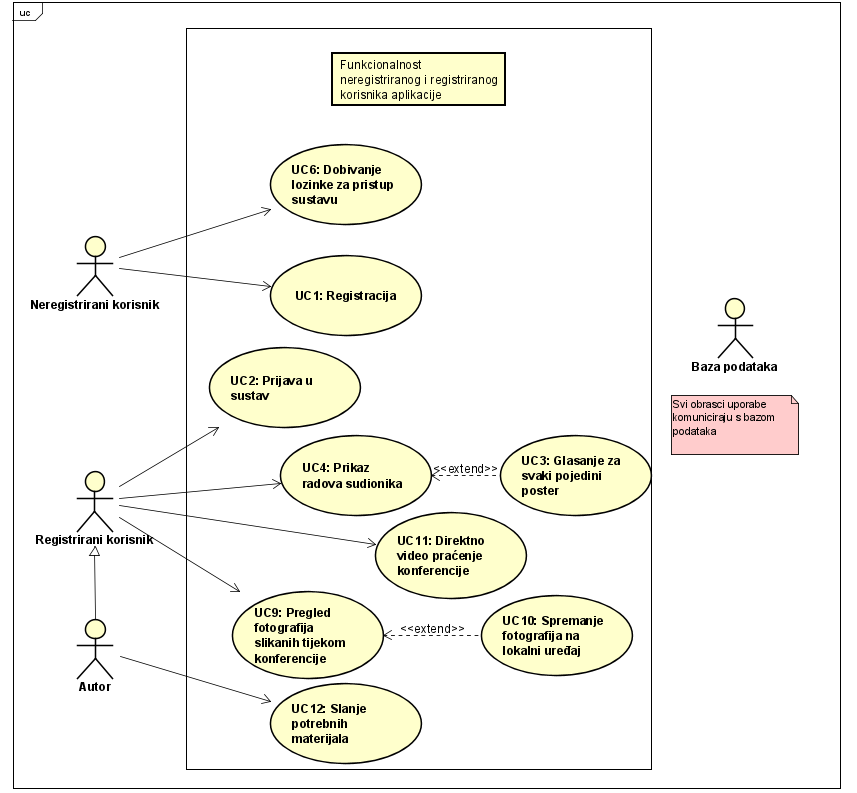
\includegraphics[scale=0.6]{slike/uc dijagram registrirani i neregistrirani korisnik.PNG} %veličina slike u odnosu na originalnu datoteku i pozicija slike
						\centering
						\caption{Dijagram obrazaca uporabe - korisnici}
						\label{fig:promjene}
					\end{figure}
				\eject		
				
			\subsection{Sekvencijski dijagrami}
				
				\textbf{\textit{dio 1. revizije}}\\
				
				\textit{Nacrtati sekvencijske dijagrame koji modeliraju najvažnije dijelove sustava (max. 4 dijagrama). Ukoliko postoji nedoumica oko odabira, razjasniti s asistentom. Uz svaki dijagram napisati detaljni opis dijagrama.}
				\eject
	
		\section{Ostali zahtjevi}
		
			\textbf{\textit{dio 1. revizije}}\\
		 
			 \textit{Nefunkcionalni zahtjevi i zahtjevi domene primjene dopunjuju funkcionalne zahtjeve. Oni opisuju \textbf{kako se sustav treba ponašati} i koja \textbf{ograničenja} treba poštivati (performanse, korisničko iskustvo, pouzdanost, standardi kvalitete, sigurnost...). Primjeri takvih zahtjeva u Vašem projektu mogu biti: podržani jezici korisničkog sučelja, vrijeme odziva, najveći mogući podržani broj korisnika, podržane web/mobilne platforme, razina zaštite (protokoli komunikacije, kriptiranje...)... Svaki takav zahtjev potrebno je navesti u jednoj ili dvije rečenice.}
			 
			 
			 
	